% --- JEPA Motivation ---
\begin{frame}{Motivation for JEPA Models}
  \begin{itemize}
    \item Most self-supervised learning (SSL) approaches focus on predicting local features or reconstructing pixels. Can we go further and predict high-level, abstract embeddings instead?
    \item \textbf{JEPA's key idea:} Predict the \textit{representations} of masked or missing regions, not just raw pixel values. This approach enables semantically rich, meaningful representations.
    \item JEPA and world models are proposed as a path to machines that internalize how the world works. By predicting abstract representations rather than details, models can focus on semantics and ignore unpredictable noise.
    \item This shift reflects a broader vision (Y. LeCun et al.): powerful architectures like Transformers, while impressive, still lack the human/animal ability to acquire deep understanding from little labeled data. Purely scaling models does not guarantee human-like world understanding.
  \end{itemize}
\end{frame}

% --- Objective-Driven AI / AMI (Turing Post figure) ---
% \begin{frame}{Objective-Driven AI: Modules for Autonomous Intelligence}
%   \begin{columns}[T,onlytextwidth]
%     \column{0.42\textwidth}
%     \begin{itemize}\itemsep0.28em
%       \item A modular stack for autonomous intelligence (expository diagram): \textbf{Configurator} routes tasks; \textbf{Perception} ingests sensors; \textbf{World model} predicts states and fills in missing information; \textbf{Actor} proposes actions; \textbf{Cost} (intrinsic + critic) scores outcomes; \textbf{short-term memory} holds recent interaction history.
%       \item \textbf{SSL} is meant to learn these components from unlabeled streams, analogous to observing the world without a label for every frame.
%       \item \textbf{Abstract representations} focus on what matters and suppress noise (cf.\ selective attention / inattentional blindness in human perception).
%     \end{itemize}
%     \column{0.56\textwidth}
%     \centering
%     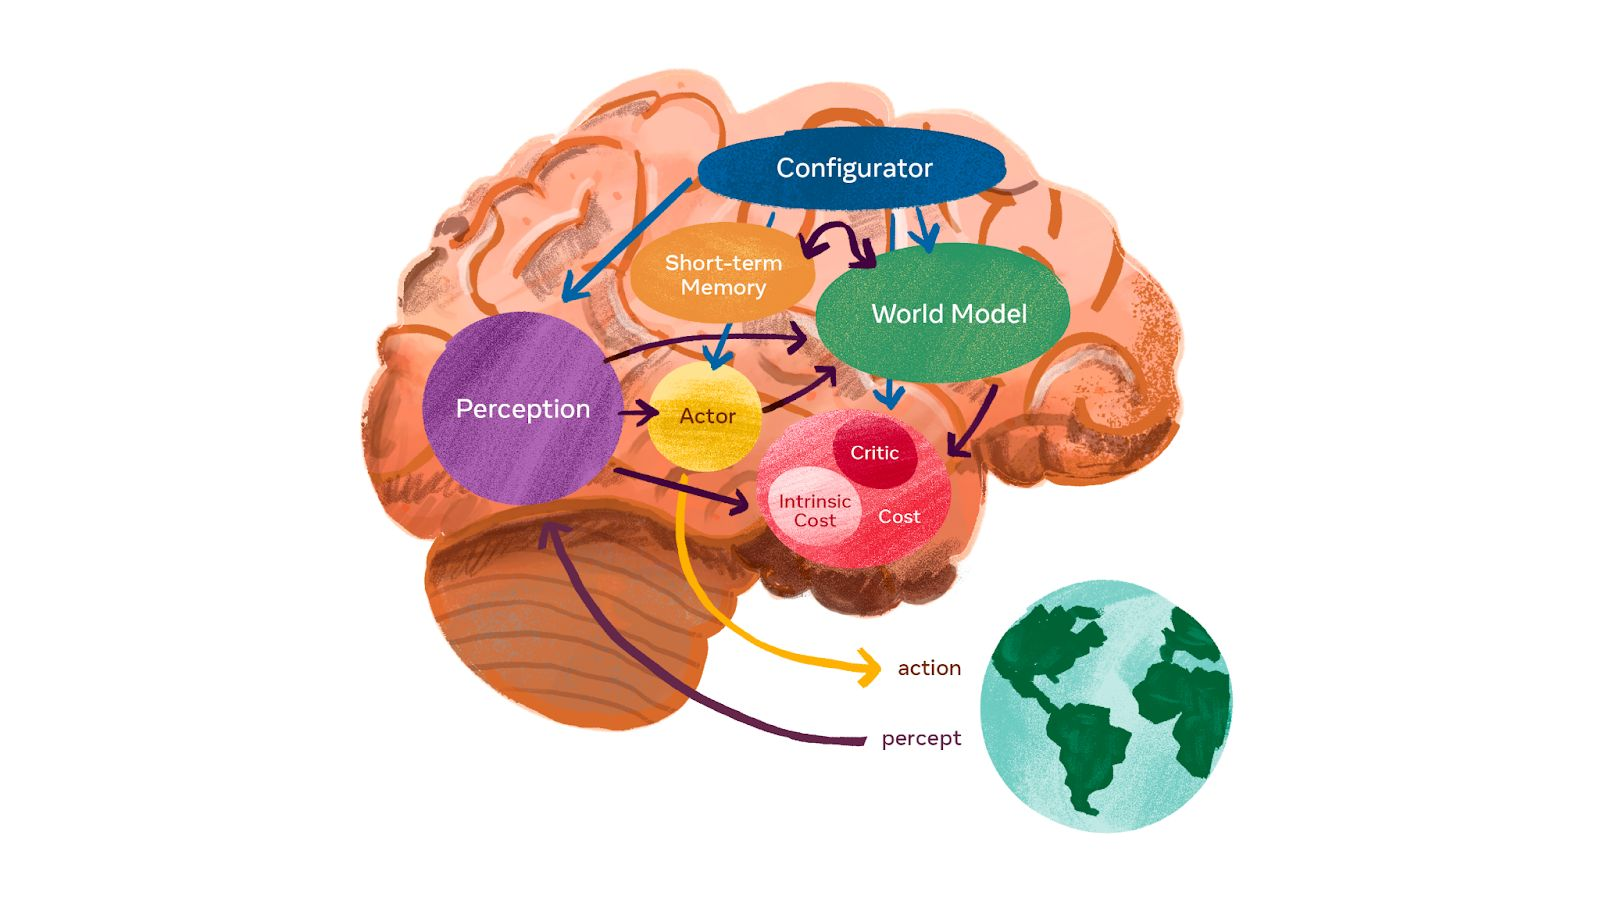
\includegraphics[width=\linewidth]{assets/New-Lecture_JEPA_models/turing_jepa_objective_driven_ami.jpg}\\[0.2em]
%     {\scriptsize Conceptual AMI diagram (figure as used in Turing Post; image credit Meta AI / Y.\ LeCun).}
%   \end{columns}
% \end{frame}

% --- What is JEPA? ---
\begin{frame}{What are Joint Embedding Predictive Architectures (JEPA)?}
  Models learns by predicting the \textbf{embedding} of one part of the input (e.g.\ a future segment or a masked region) from the representation of another (context / past), using paired encoders and a predictor.
  For example, predict the embedding of a masked image region (target) from the visible (context) regions.
  \begin{itemize}
    \item Do not reconstruct pixels; learn on the level of abstract representations.
    \item The primary training signal is in \textbf{representation space}.
    \item Concrete models include I-JEPA (images), V-JEPA (video), MC-JEPA (motion/content), and extensions to other modalities.
  \end{itemize}
  % \centering
  % 
\includegraphics[width=\textwidth,height=0.44\textheight,keepaspectratio]{images/ssl/slide_14_1_img.png}
\end{frame}

\begin{frame}{JEPA: Architecture for the World Model}
  \begin{columns}[T,onlytextwidth]
    \column{0.38\textwidth}
    \begin{itemize}
      \item \textbf{JEPA: Joint Embedding Predictive Architecture.}
      \begin{itemize}
        \item $x$: observed past and present
        \item $y$: future
        \item $a$: action
        \item $z$: latent variable (unknown)
        \item $D()$: prediction cost
        \item $C()$: surrogate cost
      \end{itemize}
    \end{itemize}
    \column{0.62\textwidth}
    \centering
    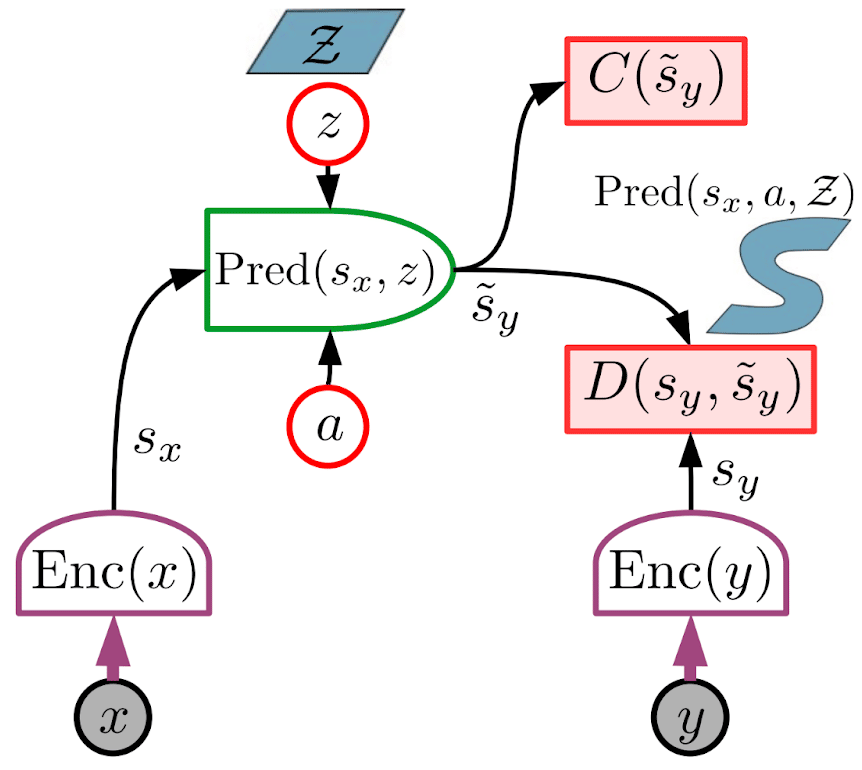
\includegraphics[width=0.8\linewidth, height=0.8\textheight, keepaspectratio]{assets/New-Lecture_JEPA_models/turing_jepa_core_predictor_diagram.png}
    \linebreak
    {\scriptsize Reference: Adapted from Turing Post / Meta AI core JEPA diagram.}
  \end{columns}
\end{frame}

% --- JEPA core world-model diagram ---
\begin{frame}{JEPA: Architecture}
  \begin{columns}[T,onlytextwidth]
    \column{0.36\textwidth}
    \begin{itemize}\itemsep0.3em
      \item Observed \textbf{$x$} (past/present) and \textbf{$y$} (future or target) map to representations \textbf{$s_x$}, \textbf{$s_y$}.
      \item A \textbf{predictor} maps $(s_x, a, z)$ to \textbf{$\tilde{s}_y$}; optional \textbf{action} $a$ and latent \textbf{$z$} capture aspects of $y$ not fixed by $x$.
      \item Training minimizes a prediction cost \textbf{$D(s_y,\tilde{s}_y)$}.
    \end{itemize}
    \column{0.62\textwidth}
    \centering
    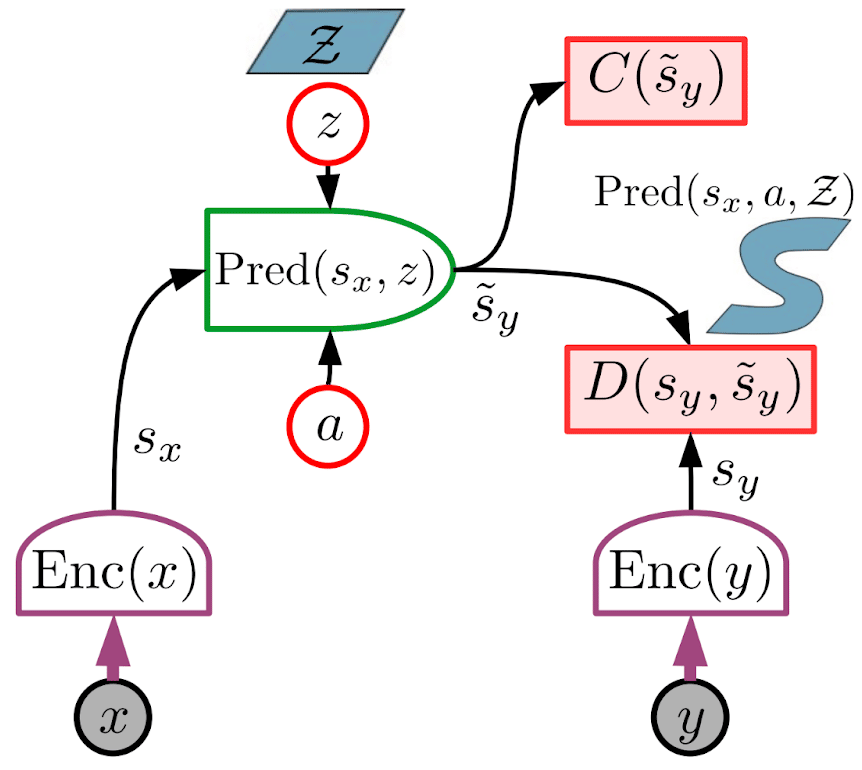
\includegraphics[width=0.8\linewidth, height=0.8\textheight, keepaspectratio]{assets/New-Lecture_JEPA_models/turing_jepa_core_predictor_diagram.png}
    \linebreak
    {\scriptsize Reference: Adapted from Turing Post / Meta AI core JEPA diagram.}
  \end{columns}
\end{frame}
% --- Multistep recurrent JEPA (Turing Post) ---
% \begin{frame}{Multistep / Recurrent World Models}
%   \begin{columns}[T,onlytextwidth]
%     \column{0.4\textwidth}
%     \begin{itemize}\itemsep0.3em
%       \item The same world model can be \textbf{unrolled} over time: each predicted state feeds the next step, with actions $a_0,a_1,\ldots$ and \textbf{guardrail} / task costs on the trajectory.
%       \item Conceptually related to \textbf{model predictive control}: optimize actions against predicted costs under learned dynamics in representation space.
%     \end{itemize}
%     \column{0.58\textwidth}
%     \centering
%     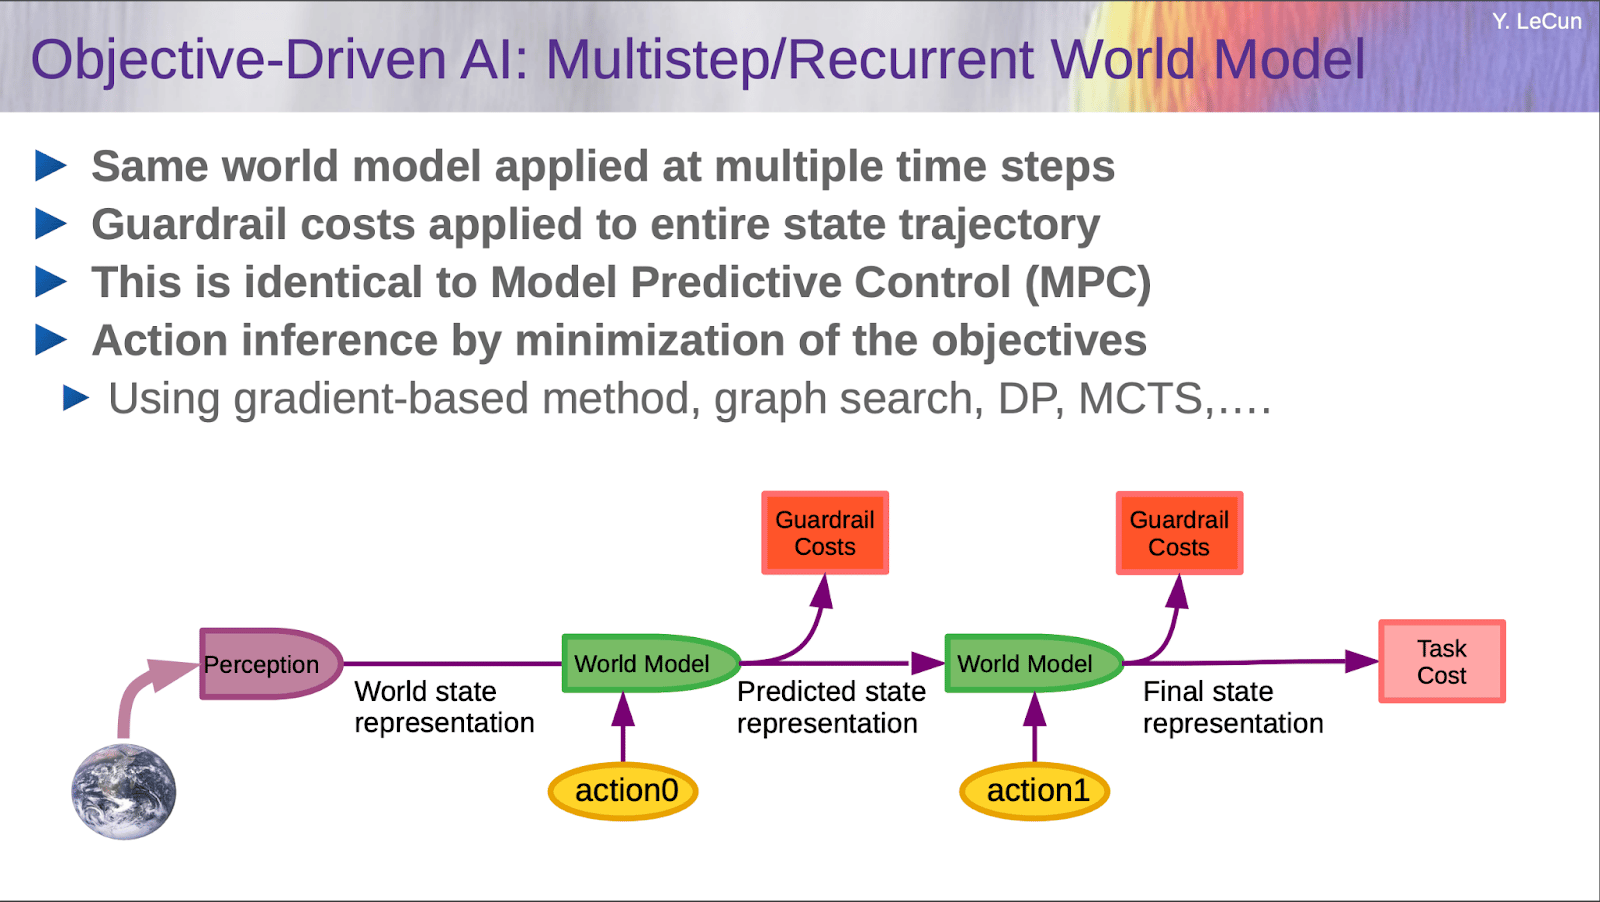
\includegraphics[width=\linewidth]{assets/New-Lecture_JEPA_models/turing_jepa_multistep_recurrent_wm.png}\\[0.2em]
%     {\scriptsize Multistep recurrent world model (Turing Post).}
%   \end{columns}
% \end{frame}

% % --- Hierarchical JEPA (Turing Post) ---
% \begin{frame}{Hierarchical World Models and Planning}
%   \begin{columns}[T,onlytextwidth]
%     \column{0.4\textwidth}
%     \begin{itemize}\itemsep0.28em
%       \item Higher levels can predict \textbf{longer horizons} in \textbf{more abstract} representations; lower levels run on shorter time scales with concrete actions.
%       \item Higher-level predictions can define \textbf{subtask objectives} for lower levels; \textbf{guardrails} at each level encode safety or constraints.
%     \end{itemize}
%     \column{0.58\textwidth}
%     \centering
%     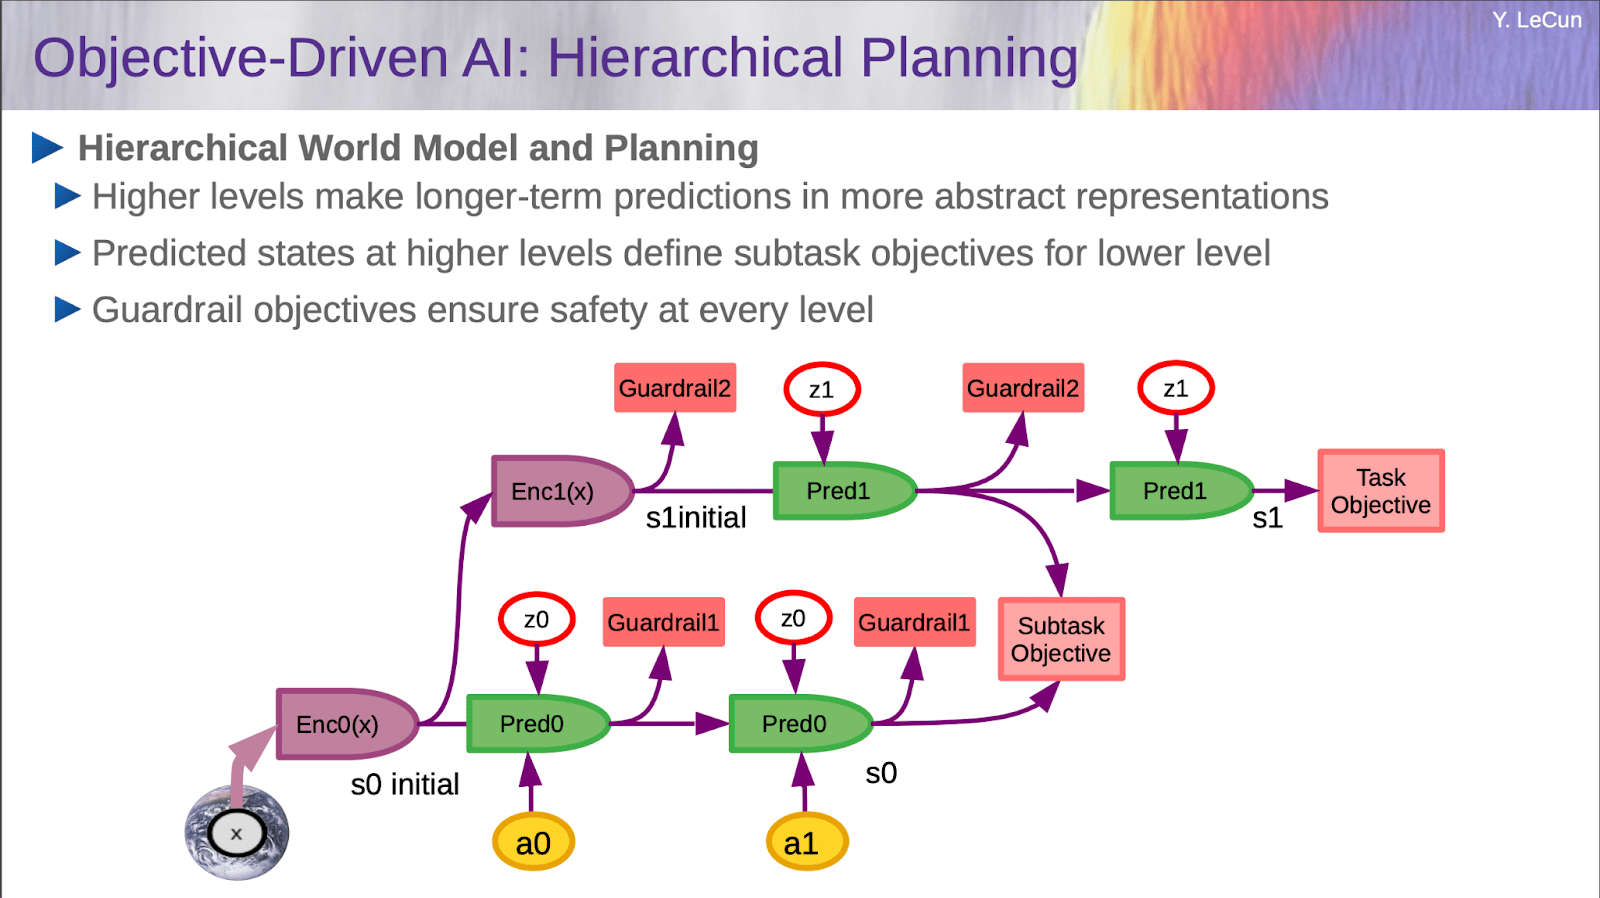
\includegraphics[width=\linewidth]{assets/New-Lecture_JEPA_models/turing_jepa_hierarchical_planning.png}\\[0.2em]
%     {\scriptsize Hierarchical planning (Turing Post).}
%   \end{columns}
% \end{frame}

